\documentclass[1p]{elsarticle_modified}
%\bibliographystyle{elsarticle-num}

%\usepackage[colorlinks]{hyperref}
%\usepackage{abbrmath_seonhwa} %\Abb, \Ascr, \Acal ,\Abf, \Afrak
\usepackage{amsfonts}
\usepackage{amssymb}
\usepackage{amsmath}
\usepackage{amsthm}
\usepackage{scalefnt}
\usepackage{amsbsy}
\usepackage{kotex}
\usepackage{caption}
\usepackage{subfig}
\usepackage{color}
\usepackage{graphicx}
\usepackage{xcolor} %% white, black, red, green, blue, cyan, magenta, yellow
\usepackage{float}
\usepackage{setspace}
\usepackage{hyperref}

\usepackage{tikz}
\usetikzlibrary{arrows}

\usepackage{multirow}
\usepackage{array} % fixed length table
\usepackage{hhline}

%%%%%%%%%%%%%%%%%%%%%
\makeatletter
\renewcommand*\env@matrix[1][\arraystretch]{%
	\edef\arraystretch{#1}%
	\hskip -\arraycolsep
	\let\@ifnextchar\new@ifnextchar
	\array{*\c@MaxMatrixCols c}}
\makeatother %https://tex.stackexchange.com/questions/14071/how-can-i-increase-the-line-spacing-in-a-matrix
%%%%%%%%%%%%%%%

\usepackage[normalem]{ulem}

\newcommand{\msout}[1]{\ifmmode\text{\sout{\ensuremath{#1}}}\else\sout{#1}\fi}
%SOURCE: \msout is \stkout macro in https://tex.stackexchange.com/questions/20609/strikeout-in-math-mode

\newcommand{\cancel}[1]{
	\ifmmode
	{\color{red}\msout{#1}}
	\else
	{\color{red}\sout{#1}}
	\fi
}

\newcommand{\add}[1]{
	{\color{blue}\uwave{#1}}
}

\newcommand{\replace}[2]{
	\ifmmode
	{\color{red}\msout{#1}}{\color{blue}\uwave{#2}}
	\else
	{\color{red}\sout{#1}}{\color{blue}\uwave{#2}}
	\fi
}

\newcommand{\Sol}{\mathcal{S}} %segment
\newcommand{\D}{D} %diagram
\newcommand{\A}{\mathcal{A}} %arc


%%%%%%%%%%%%%%%%%%%%%%%%%%%%%5 test

\def\sl{\operatorname{\textup{SL}}(2,\Cbb)}
\def\psl{\operatorname{\textup{PSL}}(2,\Cbb)}
\def\quan{\mkern 1mu \triangleright \mkern 1mu}

\theoremstyle{definition}
\newtheorem{thm}{Theorem}[section]
\newtheorem{prop}[thm]{Proposition}
\newtheorem{lem}[thm]{Lemma}
\newtheorem{ques}[thm]{Question}
\newtheorem{cor}[thm]{Corollary}
\newtheorem{defn}[thm]{Definition}
\newtheorem{exam}[thm]{Example}
\newtheorem{rmk}[thm]{Remark}
\newtheorem{alg}[thm]{Algorithm}

\newcommand{\I}{\sqrt{-1}}
\begin{document}

%\begin{frontmatter}
%
%\title{Boundary parabolic representations of knots up to 8 crossings}
%
%%% Group authors per affiliation:
%\author{Yunhi Cho} 
%\address{Department of Mathematics, University of Seoul, Seoul, Korea}
%\ead{yhcho@uos.ac.kr}
%
%
%\author{Seonhwa Kim} %\fnref{s_kim}}
%\address{Center for Geometry and Physics, Institute for Basic Science, Pohang, 37673, Korea}
%\ead{ryeona17@ibs.re.kr}
%
%\author{Hyuk Kim}
%\address{Department of Mathematical Sciences, Seoul National University, Seoul 08826, Korea}
%\ead{hyukkim@snu.ac.kr}
%
%\author{Seokbeom Yoon}
%\address{Department of Mathematical Sciences, Seoul National University, Seoul, 08826,  Korea}
%\ead{sbyoon15@snu.ac.kr}
%
%\begin{abstract}
%We find all boundary parabolic representation of knots up to 8 crossings.
%
%\end{abstract}
%\begin{keyword}
%    \MSC[2010] 57M25 
%\end{keyword}
%
%\end{frontmatter}

%\linenumbers
%\tableofcontents
%
\newcommand\colored[1]{\textcolor{white}{\rule[-0.35ex]{0.8em}{1.4ex}}\kern-0.8em\color{red} #1}%
%\newcommand\colored[1]{\textcolor{white}{ #1}\kern-2.17ex	\textcolor{white}{ #1}\kern-1.81ex	\textcolor{white}{ #1}\kern-2.15ex\color{red}#1	}

{\Large $\underline{12a_{0101}~(K12a_{0101})}$}

\setlength{\tabcolsep}{10pt}
\renewcommand{\arraystretch}{1.6}
\vspace{1cm}\begin{tabular}{m{100pt}>{\centering\arraybackslash}m{274pt}}
\multirow{5}{120pt}{
	\centering
	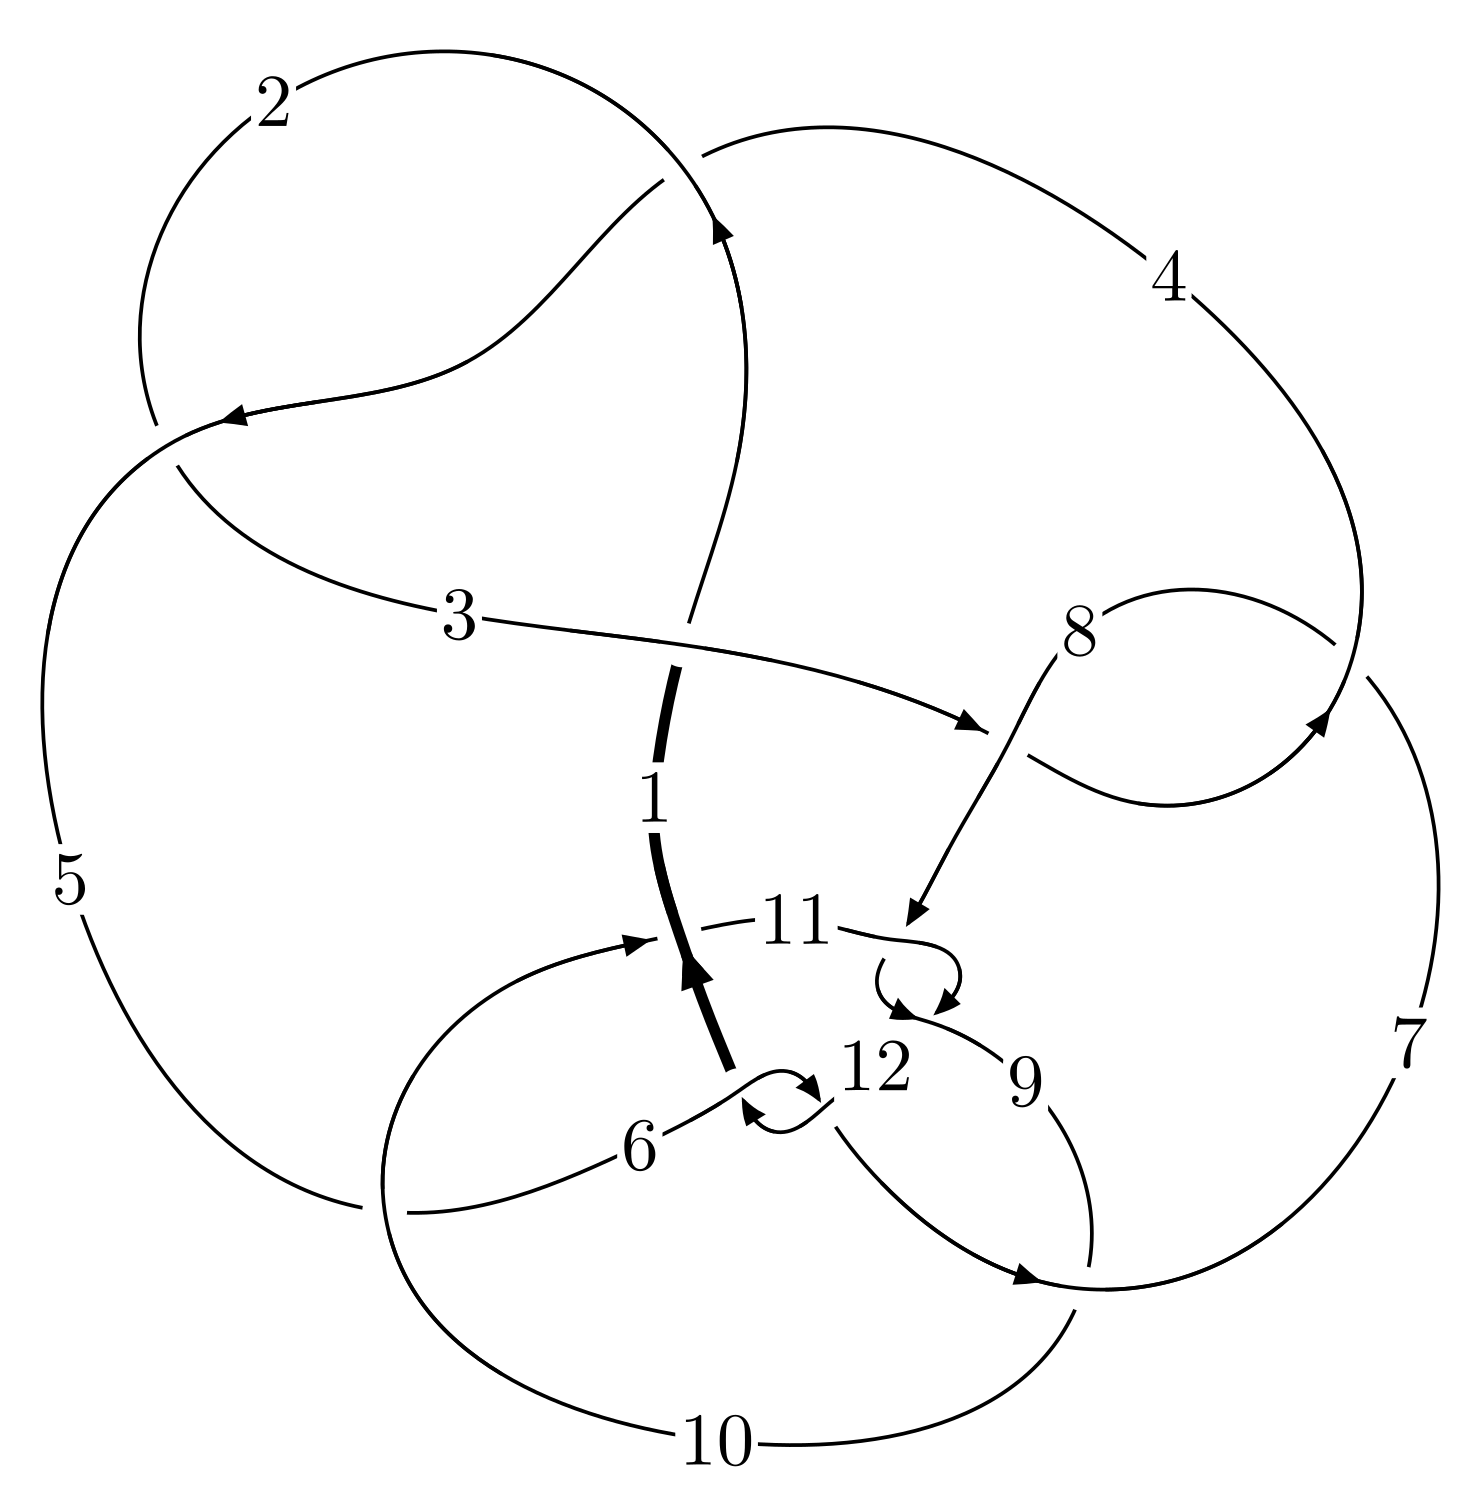
\includegraphics[width=112pt]{../../../GIT/diagram.site/Diagrams/png/902_12a_0101.png}\\
\ \ \ A knot diagram\footnotemark}&
\allowdisplaybreaks
\textbf{Linearized knot diagam} \\
\cline{2-2}
 &
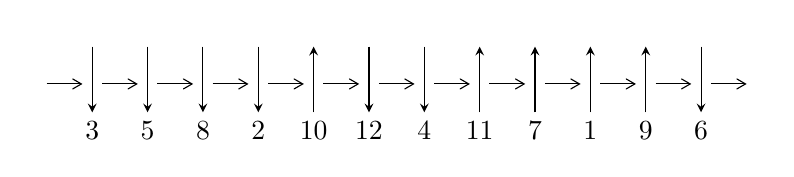
\begin{tikzpicture}[x=20pt, y=17pt]
	% nodes
	\node (C0) at (0, 0) {};
	\node (C1) at (1, 0) {};
	\node (C1U) at (1, +1) {};
	\node (C1D) at (1, -1) {3};

	\node (C2) at (2, 0) {};
	\node (C2U) at (2, +1) {};
	\node (C2D) at (2, -1) {5};

	\node (C3) at (3, 0) {};
	\node (C3U) at (3, +1) {};
	\node (C3D) at (3, -1) {8};

	\node (C4) at (4, 0) {};
	\node (C4U) at (4, +1) {};
	\node (C4D) at (4, -1) {2};

	\node (C5) at (5, 0) {};
	\node (C5U) at (5, +1) {};
	\node (C5D) at (5, -1) {10};

	\node (C6) at (6, 0) {};
	\node (C6U) at (6, +1) {};
	\node (C6D) at (6, -1) {12};

	\node (C7) at (7, 0) {};
	\node (C7U) at (7, +1) {};
	\node (C7D) at (7, -1) {4};

	\node (C8) at (8, 0) {};
	\node (C8U) at (8, +1) {};
	\node (C8D) at (8, -1) {11};

	\node (C9) at (9, 0) {};
	\node (C9U) at (9, +1) {};
	\node (C9D) at (9, -1) {7};

	\node (C10) at (10, 0) {};
	\node (C10U) at (10, +1) {};
	\node (C10D) at (10, -1) {1};

	\node (C11) at (11, 0) {};
	\node (C11U) at (11, +1) {};
	\node (C11D) at (11, -1) {9};

	\node (C12) at (12, 0) {};
	\node (C12U) at (12, +1) {};
	\node (C12D) at (12, -1) {6};
	\node (C13) at (13, 0) {};

	% arrows
	\draw[->,>={angle 60}]
	(C0) edge (C1) (C1) edge (C2) (C2) edge (C3) (C3) edge (C4) (C4) edge (C5) (C5) edge (C6) (C6) edge (C7) (C7) edge (C8) (C8) edge (C9) (C9) edge (C10) (C10) edge (C11) (C11) edge (C12) (C12) edge (C13) ;	\draw[->,>=stealth]
	(C1U) edge (C1D) (C2U) edge (C2D) (C3U) edge (C3D) (C4U) edge (C4D) (C5D) edge (C5U) (C6U) edge (C6D) (C7U) edge (C7D) (C8D) edge (C8U) (C9D) edge (C9U) (C10D) edge (C10U) (C11D) edge (C11U) (C12U) edge (C12D) ;
	\end{tikzpicture} \\
\hhline{~~} \\& 
\textbf{Solving Sequence} \\ \cline{2-2} 
 &
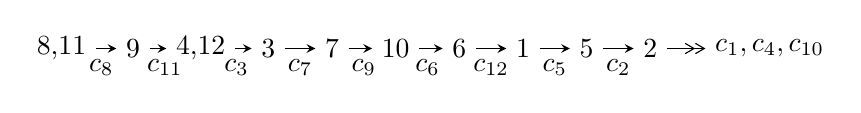
\begin{tikzpicture}[x=23pt, y=7pt]
	% node
	\node (A0) at (-1/8, 0) {8,11};
	\node (A1) at (1, 0) {9};
	\node (A2) at (33/16, 0) {4,12};
	\node (A3) at (25/8, 0) {3};
	\node (A4) at (33/8, 0) {7};
	\node (A5) at (41/8, 0) {10};
	\node (A6) at (49/8, 0) {6};
	\node (A7) at (57/8, 0) {1};
	\node (A8) at (65/8, 0) {5};
	\node (A9) at (73/8, 0) {2};
	\node (C1) at (1/2, -1) {$c_{8}$};
	\node (C2) at (3/2, -1) {$c_{11}$};
	\node (C3) at (21/8, -1) {$c_{3}$};
	\node (C4) at (29/8, -1) {$c_{7}$};
	\node (C5) at (37/8, -1) {$c_{9}$};
	\node (C6) at (45/8, -1) {$c_{6}$};
	\node (C7) at (53/8, -1) {$c_{12}$};
	\node (C8) at (61/8, -1) {$c_{5}$};
	\node (C9) at (69/8, -1) {$c_{2}$};
	\node (A10) at (11, 0) {$c_{1},c_{4},c_{10}$};

	% edge
	\draw[->,>=stealth]	
	(A0) edge (A1) (A1) edge (A2) (A2) edge (A3) (A3) edge (A4) (A4) edge (A5) (A5) edge (A6) (A6) edge (A7) (A7) edge (A8) (A8) edge (A9) ;
	\draw[->>,>={angle 60}]	
	(A9) edge (A10);
\end{tikzpicture} \\ 

\end{tabular} \\

\footnotetext{
The image of knot diagram is generated by the software ``\textbf{Draw programme}" developed by Andrew Bartholomew(\url{http://www.layer8.co.uk/maths/draw/index.htm\#Running-draw}), where we modified some parts for our purpose(\url{https://github.com/CATsTAILs/LinksPainter}).
}\phantom \\ \newline 
\centering \textbf{Ideals for irreducible components\footnotemark of $X_{\text{par}}$} 
 
\begin{align*}
I^u_{1}&=\langle 
1.17649\times10^{609} u^{124}-3.36190\times10^{609} u^{123}+\cdots+1.03048\times10^{610} b+8.64846\times10^{610},\\
\phantom{I^u_{1}}&\phantom{= \langle  }-1.13257\times10^{610} u^{124}+3.05226\times10^{610} u^{123}+\cdots+9.27430\times10^{610} a-4.30072\times10^{612},\\
\phantom{I^u_{1}}&\phantom{= \langle  }u^{125}-4 u^{124}+\cdots-2358 u-81\rangle \\
I^u_{2}&=\langle 
b,\;- u^8+2 u^7+u^6-4 u^5+u^4+2 u^3-2 u^2+a+2 u-1,\;u^9- u^8-2 u^7+3 u^6+u^5-3 u^4+2 u^3- u+1\rangle \\
I^u_{3}&=\langle 
b+3 a+2,\;9 a^2+15 a+5,\;u+1\rangle \\
\\
\end{align*}
\raggedright * 3 irreducible components of $\dim_{\mathbb{C}}=0$, with total 136 representations.\\
\footnotetext{All coefficients of polynomials are rational numbers. But the coefficients are sometimes approximated in decimal forms when there is not enough margin.}
\newpage
\renewcommand{\arraystretch}{1}
\centering \section*{I. $I^u_{1}= \langle 1.18\times10^{609} u^{124}-3.36\times10^{609} u^{123}+\cdots+1.03\times10^{610} b+8.65\times10^{610},\;-1.13\times10^{610} u^{124}+3.05\times10^{610} u^{123}+\cdots+9.27\times10^{610} a-4.30\times10^{612},\;u^{125}-4 u^{124}+\cdots-2358 u-81 \rangle$}
\flushleft \textbf{(i) Arc colorings}\\
\begin{tabular}{m{7pt} m{180pt} m{7pt} m{180pt} }
\flushright $a_{8}=$&$\begin{pmatrix}1\\0\end{pmatrix}$ \\
\flushright $a_{11}=$&$\begin{pmatrix}0\\u\end{pmatrix}$ \\
\flushright $a_{9}=$&$\begin{pmatrix}1\\- u^2\end{pmatrix}$ \\
\flushright $a_{4}=$&$\begin{pmatrix}0.122120 u^{124}-0.329110 u^{123}+\cdots+830.926 u+46.3724\\-0.114169 u^{124}+0.326247 u^{123}+\cdots-267.251 u-8.39267\end{pmatrix}$ \\
\flushright $a_{12}=$&$\begin{pmatrix}u\\- u^3+u\end{pmatrix}$ \\
\flushright $a_{3}=$&$\begin{pmatrix}0.00795030 u^{124}-0.00286248 u^{123}+\cdots+563.675 u+37.9797\\-0.114169 u^{124}+0.326247 u^{123}+\cdots-267.251 u-8.39267\end{pmatrix}$ \\
\flushright $a_{7}=$&$\begin{pmatrix}-0.0897427 u^{124}+0.263504 u^{123}+\cdots-662.051 u-35.8488\\0.165533 u^{124}-0.472119 u^{123}+\cdots+397.821 u+12.7393\end{pmatrix}$ \\
\flushright $a_{10}=$&$\begin{pmatrix}0.0447494 u^{124}-0.159277 u^{123}+\cdots-891.931 u-40.9827\\-0.0497440 u^{124}+0.142055 u^{123}+\cdots-80.7797 u-3.74242\end{pmatrix}$ \\
\flushright $a_{6}=$&$\begin{pmatrix}0.114516 u^{124}-0.320981 u^{123}+\cdots-240.354 u-21.7764\\0.107402 u^{124}-0.302520 u^{123}+\cdots+254.621 u+7.97521\end{pmatrix}$ \\
\flushright $a_{1}=$&$\begin{pmatrix}-0.0581366 u^{124}+0.249551 u^{123}+\cdots+1107.65 u+46.5213\\-0.0948218 u^{124}+0.265936 u^{123}+\cdots-149.169 u-3.89415\end{pmatrix}$ \\
\flushright $a_{5}=$&$\begin{pmatrix}0.106209 u^{124}-0.294233 u^{123}+\cdots+57.8710 u-7.77602\\0.0561392 u^{124}-0.160305 u^{123}+\cdots+133.289 u+4.09848\end{pmatrix}$ \\
\flushright $a_{2}=$&$\begin{pmatrix}0.115742 u^{124}-0.290456 u^{123}+\cdots+744.384 u+37.5680\\-0.0561392 u^{124}+0.160305 u^{123}+\cdots-133.289 u-4.09848\end{pmatrix}$\\&\end{tabular}
\flushleft \textbf{(ii) Obstruction class $= -1$}\\~\\
\flushleft \textbf{(iii) Cusp Shapes $= 0.594099 u^{124}-1.86176 u^{123}+\cdots+270.776 u-11.5444$}\\~\\
\newpage\renewcommand{\arraystretch}{1}
\flushleft \textbf{(iv) u-Polynomials at the component}\newline \\
\begin{tabular}{m{50pt}|m{274pt}}
Crossings & \hspace{64pt}u-Polynomials at each crossing \\
\hline $$\begin{aligned}c_{1}\end{aligned}$$&$\begin{aligned}
&u^{125}+63 u^{124}+\cdots+271 u+1
\end{aligned}$\\
\hline $$\begin{aligned}c_{2},c_{4}\end{aligned}$$&$\begin{aligned}
&u^{125}-11 u^{124}+\cdots-9 u-1
\end{aligned}$\\
\hline $$\begin{aligned}c_{3},c_{7}\end{aligned}$$&$\begin{aligned}
&u^{125}+2 u^{124}+\cdots+512 u+512
\end{aligned}$\\
\hline $$\begin{aligned}c_{5}\end{aligned}$$&$\begin{aligned}
&u^{125}-2 u^{124}+\cdots-756 u+324
\end{aligned}$\\
\hline $$\begin{aligned}c_{6},c_{12}\end{aligned}$$&$\begin{aligned}
&u^{125}-3 u^{124}+\cdots+3 u-1
\end{aligned}$\\
\hline $$\begin{aligned}c_{8},c_{11}\end{aligned}$$&$\begin{aligned}
&u^{125}+4 u^{124}+\cdots-2358 u+81
\end{aligned}$\\
\hline $$\begin{aligned}c_{9}\end{aligned}$$&$\begin{aligned}
&9(9 u^{125}-12 u^{124}+\cdots+2.83664\times10^{9} u+2.59859\times10^{8})
\end{aligned}$\\
\hline $$\begin{aligned}c_{10}\end{aligned}$$&$\begin{aligned}
&9(9 u^{125}-21 u^{124}+\cdots+1.22889\times10^{8} u+5290529)
\end{aligned}$\\
\hline
\end{tabular}\\~\\
\newpage\renewcommand{\arraystretch}{1}
\flushleft \textbf{(v) Riley Polynomials at the component}\newline \\
\begin{tabular}{m{50pt}|m{274pt}}
Crossings & \hspace{64pt}Riley Polynomials at each crossing \\
\hline $$\begin{aligned}c_{1}\end{aligned}$$&$\begin{aligned}
&y^{125}+9 y^{124}+\cdots+91007 y-1
\end{aligned}$\\
\hline $$\begin{aligned}c_{2},c_{4}\end{aligned}$$&$\begin{aligned}
&y^{125}-63 y^{124}+\cdots+271 y-1
\end{aligned}$\\
\hline $$\begin{aligned}c_{3},c_{7}\end{aligned}$$&$\begin{aligned}
&y^{125}+54 y^{124}+\cdots-1572864 y-262144
\end{aligned}$\\
\hline $$\begin{aligned}c_{5}\end{aligned}$$&$\begin{aligned}
&y^{125}-12 y^{124}+\cdots+16685352 y-104976
\end{aligned}$\\
\hline $$\begin{aligned}c_{6},c_{12}\end{aligned}$$&$\begin{aligned}
&y^{125}+85 y^{124}+\cdots+31 y-1
\end{aligned}$\\
\hline $$\begin{aligned}c_{8},c_{11}\end{aligned}$$&$\begin{aligned}
&y^{125}-90 y^{124}+\cdots+665982 y-6561
\end{aligned}$\\
\hline $$\begin{aligned}c_{9}\end{aligned}$$&$\begin{aligned}
&81(81 y^{125}-3294 y^{124}+\cdots+2.87254\times10^{18} y-6.75265\times10^{16})
\end{aligned}$\\
\hline $$\begin{aligned}c_{10}\end{aligned}$$&$\begin{aligned}
&81\\
&\cdot(81 y^{125}-4023 y^{124}+\cdots+7567318376329835 y-27989697099841)
\end{aligned}$\\
\hline
\end{tabular}\\~\\
\newpage\flushleft \textbf{(vi) Complex Volumes and Cusp Shapes}
$$\begin{array}{c|c|c}  
\text{Solutions to }I^u_{1}& \I (\text{vol} + \sqrt{-1}CS) & \text{Cusp shape}\\
 \hline 
\begin{aligned}
u &= \phantom{-}1.00462\phantom{ +0.000000I} \\
a &= \phantom{-}1.20830\phantom{ +0.000000I} \\
b &= -1.62729\phantom{ +0.000000I}\end{aligned}
 & -7.22833\phantom{ +0.000000I} & \phantom{-0.000000 } 0 \\ \hline\begin{aligned}
u &= -1.019800 + 0.033143 I \\
a &= -7.66625 + 0.65119 I \\
b &= -0.634089 + 0.498710 I\end{aligned}
 & \phantom{-}1.42901 - 1.00847 I & \phantom{-0.000000 } 0 \\ \hline\begin{aligned}
u &= -1.019800 - 0.033143 I \\
a &= -7.66625 - 0.65119 I \\
b &= -0.634089 - 0.498710 I\end{aligned}
 & \phantom{-}1.42901 + 1.00847 I & \phantom{-0.000000 } 0 \\ \hline\begin{aligned}
u &= \phantom{-}0.553570 + 0.776320 I \\
a &= -0.580852 - 0.370960 I \\
b &= -0.495636 + 0.814877 I\end{aligned}
 & -4.15405 + 3.73457 I & \phantom{-0.000000 } 0 \\ \hline\begin{aligned}
u &= \phantom{-}0.553570 - 0.776320 I \\
a &= -0.580852 + 0.370960 I \\
b &= -0.495636 - 0.814877 I\end{aligned}
 & -4.15405 - 3.73457 I & \phantom{-0.000000 } 0 \\ \hline\begin{aligned}
u &= -0.942125 + 0.068730 I \\
a &= \phantom{-}4.37119 + 1.11654 I \\
b &= -0.523784 + 1.069500 I\end{aligned}
 & \phantom{-}3.20788 + 5.56394 I & \phantom{-0.000000 } 0 \\ \hline\begin{aligned}
u &= -0.942125 - 0.068730 I \\
a &= \phantom{-}4.37119 - 1.11654 I \\
b &= -0.523784 - 1.069500 I\end{aligned}
 & \phantom{-}3.20788 - 5.56394 I & \phantom{-0.000000 } 0 \\ \hline\begin{aligned}
u &= -1.007240 + 0.321358 I \\
a &= -0.005539 - 0.814282 I \\
b &= \phantom{-}0.828223 - 0.376343 I\end{aligned}
 & \phantom{-}0.06073 - 2.33875 I & \phantom{-0.000000 } 0 \\ \hline\begin{aligned}
u &= -1.007240 - 0.321358 I \\
a &= -0.005539 + 0.814282 I \\
b &= \phantom{-}0.828223 + 0.376343 I\end{aligned}
 & \phantom{-}0.06073 + 2.33875 I & \phantom{-0.000000 } 0 \\ \hline\begin{aligned}
u &= -0.185640 + 0.922819 I \\
a &= -0.853594 - 0.485251 I \\
b &= -0.750828 + 0.154017 I\end{aligned}
 & \phantom{-}1.33029 - 2.74208 I & \phantom{-0.000000 } 0\\
 \hline 
 \end{array}$$\newpage$$\begin{array}{c|c|c}  
\text{Solutions to }I^u_{1}& \I (\text{vol} + \sqrt{-1}CS) & \text{Cusp shape}\\
 \hline 
\begin{aligned}
u &= -0.185640 - 0.922819 I \\
a &= -0.853594 + 0.485251 I \\
b &= -0.750828 - 0.154017 I\end{aligned}
 & \phantom{-}1.33029 + 2.74208 I & \phantom{-0.000000 } 0 \\ \hline\begin{aligned}
u &= \phantom{-}0.116638 + 0.927275 I \\
a &= -0.451443 + 0.206067 I \\
b &= -0.675422 - 1.130710 I\end{aligned}
 & -1.80399 - 8.86816 I & \phantom{-0.000000 } 0 \\ \hline\begin{aligned}
u &= \phantom{-}0.116638 - 0.927275 I \\
a &= -0.451443 - 0.206067 I \\
b &= -0.675422 + 1.130710 I\end{aligned}
 & -1.80399 + 8.86816 I & \phantom{-0.000000 } 0 \\ \hline\begin{aligned}
u &= -0.897003 + 0.223487 I \\
a &= \phantom{-}2.41978 - 2.54927 I \\
b &= \phantom{-}0.327090 + 0.526695 I\end{aligned}
 & -0.596246 - 0.416978 I & \phantom{-0.000000 } 0 \\ \hline\begin{aligned}
u &= -0.897003 - 0.223487 I \\
a &= \phantom{-}2.41978 + 2.54927 I \\
b &= \phantom{-}0.327090 - 0.526695 I\end{aligned}
 & -0.596246 + 0.416978 I & \phantom{-0.000000 } 0 \\ \hline\begin{aligned}
u &= \phantom{-}0.882115 + 0.621544 I \\
a &= \phantom{-}0.394622 + 0.050709 I \\
b &= -0.277864 - 0.645271 I\end{aligned}
 & -3.17582 + 1.37189 I & \phantom{-0.000000 } 0 \\ \hline\begin{aligned}
u &= \phantom{-}0.882115 - 0.621544 I \\
a &= \phantom{-}0.394622 - 0.050709 I \\
b &= -0.277864 + 0.645271 I\end{aligned}
 & -3.17582 - 1.37189 I & \phantom{-0.000000 } 0 \\ \hline\begin{aligned}
u &= -0.679856 + 0.613009 I \\
a &= -0.028106 - 0.438962 I \\
b &= \phantom{-}0.442173 - 1.054840 I\end{aligned}
 & \phantom{-}1.15542 + 3.12032 I & \phantom{-0.000000 } 0 \\ \hline\begin{aligned}
u &= -0.679856 - 0.613009 I \\
a &= -0.028106 + 0.438962 I \\
b &= \phantom{-}0.442173 + 1.054840 I\end{aligned}
 & \phantom{-}1.15542 - 3.12032 I & \phantom{-0.000000 } 0 \\ \hline\begin{aligned}
u &= \phantom{-}1.015900 + 0.407589 I \\
a &= \phantom{-}0.100594 + 0.423342 I \\
b &= \phantom{-}0.599973 - 0.683518 I\end{aligned}
 & \phantom{-}1.14990 + 7.95106 I & \phantom{-0.000000 } 0\\
 \hline 
 \end{array}$$\newpage$$\begin{array}{c|c|c}  
\text{Solutions to }I^u_{1}& \I (\text{vol} + \sqrt{-1}CS) & \text{Cusp shape}\\
 \hline 
\begin{aligned}
u &= \phantom{-}1.015900 - 0.407589 I \\
a &= \phantom{-}0.100594 - 0.423342 I \\
b &= \phantom{-}0.599973 + 0.683518 I\end{aligned}
 & \phantom{-}1.14990 - 7.95106 I & \phantom{-0.000000 } 0 \\ \hline\begin{aligned}
u &= -1.106370 + 0.091912 I \\
a &= -0.07489 + 1.53113 I \\
b &= -0.699810 - 0.253258 I\end{aligned}
 & \phantom{-}0.621061 + 0.585081 I & \phantom{-0.000000 } 0 \\ \hline\begin{aligned}
u &= -1.106370 - 0.091912 I \\
a &= -0.07489 - 1.53113 I \\
b &= -0.699810 + 0.253258 I\end{aligned}
 & \phantom{-}0.621061 - 0.585081 I & \phantom{-0.000000 } 0 \\ \hline\begin{aligned}
u &= -0.068597 + 1.117030 I \\
a &= \phantom{-}0.747329 - 1.138740 I \\
b &= \phantom{-}0.422750 + 0.821064 I\end{aligned}
 & -1.03348 - 4.20848 I & \phantom{-0.000000 } 0 \\ \hline\begin{aligned}
u &= -0.068597 - 1.117030 I \\
a &= \phantom{-}0.747329 + 1.138740 I \\
b &= \phantom{-}0.422750 - 0.821064 I\end{aligned}
 & -1.03348 + 4.20848 I & \phantom{-0.000000 } 0 \\ \hline\begin{aligned}
u &= \phantom{-}0.492983 + 0.726321 I \\
a &= -0.733517 - 0.012243 I \\
b &= \phantom{-}0.235520 + 0.777319 I\end{aligned}
 & -0.40273 - 3.66473 I & \phantom{-0.000000 } 0 \\ \hline\begin{aligned}
u &= \phantom{-}0.492983 - 0.726321 I \\
a &= -0.733517 + 0.012243 I \\
b &= \phantom{-}0.235520 - 0.777319 I\end{aligned}
 & -0.40273 + 3.66473 I & \phantom{-0.000000 } 0 \\ \hline\begin{aligned}
u &= -0.877189\phantom{ +0.000000I} \\
a &= -0.512937\phantom{ +0.000000I} \\
b &= -0.239647\phantom{ +0.000000I}\end{aligned}
 & \phantom{-}1.26613\phantom{ +0.000000I} & \phantom{-0.000000 } 0 \\ \hline\begin{aligned}
u &= \phantom{-}0.301986 + 1.083050 I \\
a &= \phantom{-}0.658017 + 0.117846 I \\
b &= \phantom{-}0.413672 - 0.836934 I\end{aligned}
 & -0.983702 - 0.642828 I & \phantom{-0.000000 } 0 \\ \hline\begin{aligned}
u &= \phantom{-}0.301986 - 1.083050 I \\
a &= \phantom{-}0.658017 - 0.117846 I \\
b &= \phantom{-}0.413672 + 0.836934 I\end{aligned}
 & -0.983702 + 0.642828 I & \phantom{-0.000000 } 0\\
 \hline 
 \end{array}$$\newpage$$\begin{array}{c|c|c}  
\text{Solutions to }I^u_{1}& \I (\text{vol} + \sqrt{-1}CS) & \text{Cusp shape}\\
 \hline 
\begin{aligned}
u &= \phantom{-}1.120200 + 0.229947 I \\
a &= -0.611354 + 0.118039 I \\
b &= \phantom{-}1.185770 + 0.210987 I\end{aligned}
 & \phantom{-}0.98816 + 1.89695 I & \phantom{-0.000000 } 0 \\ \hline\begin{aligned}
u &= \phantom{-}1.120200 - 0.229947 I \\
a &= -0.611354 - 0.118039 I \\
b &= \phantom{-}1.185770 - 0.210987 I\end{aligned}
 & \phantom{-}0.98816 - 1.89695 I & \phantom{-0.000000 } 0 \\ \hline\begin{aligned}
u &= \phantom{-}1.169660 + 0.122507 I \\
a &= \phantom{-}0.21593 - 1.74311 I \\
b &= \phantom{-}0.585773 + 1.136850 I\end{aligned}
 & \phantom{-}2.57218 + 2.94748 I & \phantom{-0.000000 } 0 \\ \hline\begin{aligned}
u &= \phantom{-}1.169660 - 0.122507 I \\
a &= \phantom{-}0.21593 + 1.74311 I \\
b &= \phantom{-}0.585773 - 1.136850 I\end{aligned}
 & \phantom{-}2.57218 - 2.94748 I & \phantom{-0.000000 } 0 \\ \hline\begin{aligned}
u &= \phantom{-}1.177470 + 0.040674 I \\
a &= -0.451479 + 0.498059 I \\
b &= \phantom{-}1.212360 - 0.646222 I\end{aligned}
 & \phantom{-}3.33646 - 0.19030 I & \phantom{-0.000000 } 0 \\ \hline\begin{aligned}
u &= \phantom{-}1.177470 - 0.040674 I \\
a &= -0.451479 - 0.498059 I \\
b &= \phantom{-}1.212360 + 0.646222 I\end{aligned}
 & \phantom{-}3.33646 + 0.19030 I & \phantom{-0.000000 } 0 \\ \hline\begin{aligned}
u &= \phantom{-}1.129450 + 0.338053 I \\
a &= -0.66428 - 2.18288 I \\
b &= -0.380832 + 1.099280 I\end{aligned}
 & -1.50629 + 4.23005 I & \phantom{-0.000000 } 0 \\ \hline\begin{aligned}
u &= \phantom{-}1.129450 - 0.338053 I \\
a &= -0.66428 + 2.18288 I \\
b &= -0.380832 - 1.099280 I\end{aligned}
 & -1.50629 - 4.23005 I & \phantom{-0.000000 } 0 \\ \hline\begin{aligned}
u &= -1.122780 + 0.361086 I \\
a &= -1.36902 + 1.80748 I \\
b &= -0.349086 - 1.109990 I\end{aligned}
 & \phantom{-}4.36419 - 2.43164 I & \phantom{-0.000000 } 0 \\ \hline\begin{aligned}
u &= -1.122780 - 0.361086 I \\
a &= -1.36902 - 1.80748 I \\
b &= -0.349086 + 1.109990 I\end{aligned}
 & \phantom{-}4.36419 + 2.43164 I & \phantom{-0.000000 } 0\\
 \hline 
 \end{array}$$\newpage$$\begin{array}{c|c|c}  
\text{Solutions to }I^u_{1}& \I (\text{vol} + \sqrt{-1}CS) & \text{Cusp shape}\\
 \hline 
\begin{aligned}
u &= -1.148820 + 0.276283 I \\
a &= \phantom{-}0.363713 + 0.676943 I \\
b &= \phantom{-}0.234925 + 0.344834 I\end{aligned}
 & \phantom{-}4.30327 - 1.14568 I & \phantom{-0.000000 } 0 \\ \hline\begin{aligned}
u &= -1.148820 - 0.276283 I \\
a &= \phantom{-}0.363713 - 0.676943 I \\
b &= \phantom{-}0.234925 - 0.344834 I\end{aligned}
 & \phantom{-}4.30327 + 1.14568 I & \phantom{-0.000000 } 0 \\ \hline\begin{aligned}
u &= \phantom{-}0.041879 + 0.816044 I \\
a &= \phantom{-}0.269286 - 0.269487 I \\
b &= \phantom{-}0.505552 + 1.083710 I\end{aligned}
 & \phantom{-}0.63717 - 3.65490 I & \phantom{-0.000000 } 0 \\ \hline\begin{aligned}
u &= \phantom{-}0.041879 - 0.816044 I \\
a &= \phantom{-}0.269286 + 0.269487 I \\
b &= \phantom{-}0.505552 - 1.083710 I\end{aligned}
 & \phantom{-}0.63717 + 3.65490 I & \phantom{-0.000000 } 0 \\ \hline\begin{aligned}
u &= -1.103650 + 0.458723 I \\
a &= \phantom{-}1.44919 - 1.57677 I \\
b &= \phantom{-}0.581083 + 1.144450 I\end{aligned}
 & \phantom{-}2.41939 - 7.59298 I & \phantom{-0.000000 } 0 \\ \hline\begin{aligned}
u &= -1.103650 - 0.458723 I \\
a &= \phantom{-}1.44919 + 1.57677 I \\
b &= \phantom{-}0.581083 - 1.144450 I\end{aligned}
 & \phantom{-}2.41939 + 7.59298 I & \phantom{-0.000000 } 0 \\ \hline\begin{aligned}
u &= -0.790545 + 0.019933 I \\
a &= -2.56910 + 1.61319 I \\
b &= \phantom{-}0.189225 + 0.989929 I\end{aligned}
 & \phantom{-}4.85915 - 0.90928 I & \phantom{-0.000000 } 0 \\ \hline\begin{aligned}
u &= -0.790545 - 0.019933 I \\
a &= -2.56910 - 1.61319 I \\
b &= \phantom{-}0.189225 - 0.989929 I\end{aligned}
 & \phantom{-}4.85915 + 0.90928 I & \phantom{-0.000000 } 0 \\ \hline\begin{aligned}
u &= \phantom{-}1.202640 + 0.156735 I \\
a &= \phantom{-}0.32002 + 1.71886 I \\
b &= \phantom{-}0.79848 - 1.26772 I\end{aligned}
 & \phantom{-}5.49346 + 7.52898 I & \phantom{-0.000000 } 0 \\ \hline\begin{aligned}
u &= \phantom{-}1.202640 - 0.156735 I \\
a &= \phantom{-}0.32002 - 1.71886 I \\
b &= \phantom{-}0.79848 + 1.26772 I\end{aligned}
 & \phantom{-}5.49346 - 7.52898 I & \phantom{-0.000000 } 0\\
 \hline 
 \end{array}$$\newpage$$\begin{array}{c|c|c}  
\text{Solutions to }I^u_{1}& \I (\text{vol} + \sqrt{-1}CS) & \text{Cusp shape}\\
 \hline 
\begin{aligned}
u &= -1.210680 + 0.161896 I \\
a &= -0.85895 + 2.04089 I \\
b &= \phantom{-}0.248400 - 1.101470 I\end{aligned}
 & \phantom{-}4.76652 + 0.18641 I & \phantom{-0.000000 } 0 \\ \hline\begin{aligned}
u &= -1.210680 - 0.161896 I \\
a &= -0.85895 - 2.04089 I \\
b &= \phantom{-}0.248400 + 1.101470 I\end{aligned}
 & \phantom{-}4.76652 - 0.18641 I & \phantom{-0.000000 } 0 \\ \hline\begin{aligned}
u &= -0.093015 + 1.226720 I \\
a &= \phantom{-}0.818202 + 0.177043 I \\
b &= \phantom{-}0.962365 - 0.485559 I\end{aligned}
 & -0.31912 - 6.67340 I & \phantom{-0.000000 } 0 \\ \hline\begin{aligned}
u &= -0.093015 - 1.226720 I \\
a &= \phantom{-}0.818202 - 0.177043 I \\
b &= \phantom{-}0.962365 + 0.485559 I\end{aligned}
 & -0.31912 + 6.67340 I & \phantom{-0.000000 } 0 \\ \hline\begin{aligned}
u &= \phantom{-}1.244620 + 0.045072 I \\
a &= -0.21770 - 1.70656 I \\
b &= -0.69181 + 1.30600 I\end{aligned}
 & \phantom{-}8.30974 + 1.49559 I & \phantom{-0.000000 } 0 \\ \hline\begin{aligned}
u &= \phantom{-}1.244620 - 0.045072 I \\
a &= -0.21770 + 1.70656 I \\
b &= -0.69181 - 1.30600 I\end{aligned}
 & \phantom{-}8.30974 - 1.49559 I & \phantom{-0.000000 } 0 \\ \hline\begin{aligned}
u &= \phantom{-}1.187700 + 0.381857 I \\
a &= \phantom{-}0.554894 - 0.073688 I \\
b &= -1.156140 - 0.507162 I\end{aligned}
 & -0.51148 + 7.10641 I & \phantom{-0.000000 } 0 \\ \hline\begin{aligned}
u &= \phantom{-}1.187700 - 0.381857 I \\
a &= \phantom{-}0.554894 + 0.073688 I \\
b &= -1.156140 + 0.507162 I\end{aligned}
 & -0.51148 - 7.10641 I & \phantom{-0.000000 } 0 \\ \hline\begin{aligned}
u &= \phantom{-}0.160915 + 0.733050 I \\
a &= -1.081860 - 0.619622 I \\
b &= -0.918385 + 0.543413 I\end{aligned}
 & -3.67094 - 2.96823 I & \phantom{-0.000000 } 0 \\ \hline\begin{aligned}
u &= \phantom{-}0.160915 - 0.733050 I \\
a &= -1.081860 + 0.619622 I \\
b &= -0.918385 - 0.543413 I\end{aligned}
 & -3.67094 + 2.96823 I & \phantom{-0.000000 } 0\\
 \hline 
 \end{array}$$\newpage$$\begin{array}{c|c|c}  
\text{Solutions to }I^u_{1}& \I (\text{vol} + \sqrt{-1}CS) & \text{Cusp shape}\\
 \hline 
\begin{aligned}
u &= \phantom{-}1.232930 + 0.206914 I \\
a &= \phantom{-}0.297530 - 0.400461 I \\
b &= -1.112620 + 0.422938 I\end{aligned}
 & \phantom{-}5.54144 + 5.18578 I & \phantom{-0.000000 } 0 \\ \hline\begin{aligned}
u &= \phantom{-}1.232930 - 0.206914 I \\
a &= \phantom{-}0.297530 + 0.400461 I \\
b &= -1.112620 - 0.422938 I\end{aligned}
 & \phantom{-}5.54144 - 5.18578 I & \phantom{-0.000000 } 0 \\ \hline\begin{aligned}
u &= -1.250040 + 0.092802 I \\
a &= \phantom{-}0.72374 - 1.97517 I \\
b &= -0.521373 + 1.124290 I\end{aligned}
 & \phantom{-}3.12453 + 5.20896 I & \phantom{-0.000000 } 0 \\ \hline\begin{aligned}
u &= -1.250040 - 0.092802 I \\
a &= \phantom{-}0.72374 + 1.97517 I \\
b &= -0.521373 - 1.124290 I\end{aligned}
 & \phantom{-}3.12453 - 5.20896 I & \phantom{-0.000000 } 0 \\ \hline\begin{aligned}
u &= -0.412931 + 0.603388 I \\
a &= -0.095407 + 0.251832 I \\
b &= -0.080750 + 1.051060 I\end{aligned}
 & \phantom{-}2.33153 - 1.50993 I & \phantom{-0.000000 } 0 \\ \hline\begin{aligned}
u &= -0.412931 - 0.603388 I \\
a &= -0.095407 - 0.251832 I \\
b &= -0.080750 - 1.051060 I\end{aligned}
 & \phantom{-}2.33153 + 1.50993 I & \phantom{-0.000000 } 0 \\ \hline\begin{aligned}
u &= \phantom{-}1.290240 + 0.072671 I \\
a &= \phantom{-}0.10997 + 1.96088 I \\
b &= \phantom{-}0.09910 - 1.49843 I\end{aligned}
 & \phantom{-}7.75260 + 3.19534 I & \phantom{-0.000000 } 0 \\ \hline\begin{aligned}
u &= \phantom{-}1.290240 - 0.072671 I \\
a &= \phantom{-}0.10997 - 1.96088 I \\
b &= \phantom{-}0.09910 + 1.49843 I\end{aligned}
 & \phantom{-}7.75260 - 3.19534 I & \phantom{-0.000000 } 0 \\ \hline\begin{aligned}
u &= \phantom{-}0.244690 + 0.651544 I \\
a &= -0.393078 + 0.825816 I \\
b &= -0.532227 - 0.797562 I\end{aligned}
 & -4.18791 - 0.46329 I & \phantom{-0.000000 } 0 \\ \hline\begin{aligned}
u &= \phantom{-}0.244690 - 0.651544 I \\
a &= -0.393078 - 0.825816 I \\
b &= -0.532227 + 0.797562 I\end{aligned}
 & -4.18791 + 0.46329 I & \phantom{-0.000000 } 0\\
 \hline 
 \end{array}$$\newpage$$\begin{array}{c|c|c}  
\text{Solutions to }I^u_{1}& \I (\text{vol} + \sqrt{-1}CS) & \text{Cusp shape}\\
 \hline 
\begin{aligned}
u &= -0.581513 + 1.178610 I \\
a &= \phantom{-}0.126337 + 0.538620 I \\
b &= \phantom{-}0.064934 - 1.160180 I\end{aligned}
 & \phantom{-}5.99018 - 4.39123 I & \phantom{-0.000000 } 0 \\ \hline\begin{aligned}
u &= -0.581513 - 1.178610 I \\
a &= \phantom{-}0.126337 - 0.538620 I \\
b &= \phantom{-}0.064934 + 1.160180 I\end{aligned}
 & \phantom{-}5.99018 + 4.39123 I & \phantom{-0.000000 } 0 \\ \hline\begin{aligned}
u &= \phantom{-}1.267760 + 0.400092 I \\
a &= \phantom{-}0.65528 + 1.83753 I \\
b &= \phantom{-}0.60524 - 1.28225 I\end{aligned}
 & \phantom{-}4.45793 + 8.07080 I & \phantom{-0.000000 } 0 \\ \hline\begin{aligned}
u &= \phantom{-}1.267760 - 0.400092 I \\
a &= \phantom{-}0.65528 - 1.83753 I \\
b &= \phantom{-}0.60524 + 1.28225 I\end{aligned}
 & \phantom{-}4.45793 - 8.07080 I & \phantom{-0.000000 } 0 \\ \hline\begin{aligned}
u &= \phantom{-}1.204790 + 0.577085 I \\
a &= -0.241931 - 0.008506 I \\
b &= \phantom{-}0.349910 + 0.596945 I\end{aligned}
 & \phantom{-}1.92234 + 6.42207 I & \phantom{-0.000000 } 0 \\ \hline\begin{aligned}
u &= \phantom{-}1.204790 - 0.577085 I \\
a &= -0.241931 + 0.008506 I \\
b &= \phantom{-}0.349910 - 0.596945 I\end{aligned}
 & \phantom{-}1.92234 - 6.42207 I & \phantom{-0.000000 } 0 \\ \hline\begin{aligned}
u &= -0.157172 + 1.342160 I \\
a &= -0.519932 + 0.623225 I \\
b &= -0.492797 - 1.146900 I\end{aligned}
 & \phantom{-}4.19431 - 7.27901 I & \phantom{-0.000000 } 0 \\ \hline\begin{aligned}
u &= -0.157172 - 1.342160 I \\
a &= -0.519932 - 0.623225 I \\
b &= -0.492797 + 1.146900 I\end{aligned}
 & \phantom{-}4.19431 + 7.27901 I & \phantom{-0.000000 } 0 \\ \hline\begin{aligned}
u &= \phantom{-}1.274590 + 0.475627 I \\
a &= -0.76131 - 1.73414 I \\
b &= -0.75063 + 1.23502 I\end{aligned}
 & \phantom{-}1.84566 + 13.92260 I & \phantom{-0.000000 } 0 \\ \hline\begin{aligned}
u &= \phantom{-}1.274590 - 0.475627 I \\
a &= -0.76131 + 1.73414 I \\
b &= -0.75063 - 1.23502 I\end{aligned}
 & \phantom{-}1.84566 - 13.92260 I & \phantom{-0.000000 } 0\\
 \hline 
 \end{array}$$\newpage$$\begin{array}{c|c|c}  
\text{Solutions to }I^u_{1}& \I (\text{vol} + \sqrt{-1}CS) & \text{Cusp shape}\\
 \hline 
\begin{aligned}
u &= -0.212427 + 0.597178 I \\
a &= -0.79710 - 1.31566 I \\
b &= -0.675342 - 0.102623 I\end{aligned}
 & \phantom{-}1.33240 - 2.49877 I & \phantom{-0.000000 -}0. + 4.74869 I \\ \hline\begin{aligned}
u &= -0.212427 - 0.597178 I \\
a &= -0.79710 + 1.31566 I \\
b &= -0.675342 + 0.102623 I\end{aligned}
 & \phantom{-}1.33240 + 2.49877 I & \phantom{-0.000000 } 0. - 4.74869 I \\ \hline\begin{aligned}
u &= -0.865830 + 1.116940 I \\
a &= -0.279168 - 0.263603 I \\
b &= -0.375408 + 1.108420 I\end{aligned}
 & \phantom{-}5.08150 + 0.59588 I & \phantom{-0.000000 } 0 \\ \hline\begin{aligned}
u &= -0.865830 - 1.116940 I \\
a &= -0.279168 + 0.263603 I \\
b &= -0.375408 - 1.108420 I\end{aligned}
 & \phantom{-}5.08150 - 0.59588 I & \phantom{-0.000000 } 0 \\ \hline\begin{aligned}
u &= -0.057273 + 1.412250 I \\
a &= \phantom{-}0.651883 - 0.489377 I \\
b &= \phantom{-}0.670642 + 1.165170 I\end{aligned}
 & \phantom{-}1.83437 - 12.66320 I & \phantom{-0.000000 } 0 \\ \hline\begin{aligned}
u &= -0.057273 - 1.412250 I \\
a &= \phantom{-}0.651883 + 0.489377 I \\
b &= \phantom{-}0.670642 - 1.165170 I\end{aligned}
 & \phantom{-}1.83437 + 12.66320 I & \phantom{-0.000000 } 0 \\ \hline\begin{aligned}
u &= \phantom{-}0.333290 + 0.446397 I \\
a &= \phantom{-}0.481540 + 1.142050 I \\
b &= \phantom{-}0.666834 - 0.423916 I\end{aligned}
 & -1.37803 + 0.83267 I & -5.49260 - 3.40594 I \\ \hline\begin{aligned}
u &= \phantom{-}0.333290 - 0.446397 I \\
a &= \phantom{-}0.481540 - 1.142050 I \\
b &= \phantom{-}0.666834 + 0.423916 I\end{aligned}
 & -1.37803 - 0.83267 I & -5.49260 + 3.40594 I \\ \hline\begin{aligned}
u &= \phantom{-}1.37538 + 0.44635 I \\
a &= \phantom{-}0.302307 - 0.183909 I \\
b &= -1.090330 - 0.256832 I\end{aligned}
 & \phantom{-}6.12909 + 7.71732 I & \phantom{-0.000000 } 0 \\ \hline\begin{aligned}
u &= \phantom{-}1.37538 - 0.44635 I \\
a &= \phantom{-}0.302307 + 0.183909 I \\
b &= -1.090330 + 0.256832 I\end{aligned}
 & \phantom{-}6.12909 - 7.71732 I & \phantom{-0.000000 } 0\\
 \hline 
 \end{array}$$\newpage$$\begin{array}{c|c|c}  
\text{Solutions to }I^u_{1}& \I (\text{vol} + \sqrt{-1}CS) & \text{Cusp shape}\\
 \hline 
\begin{aligned}
u &= \phantom{-}1.44585 + 0.24233 I \\
a &= \phantom{-}0.12542 + 1.74268 I \\
b &= -0.15570 - 1.44249 I\end{aligned}
 & \phantom{-}12.41370 + 3.14260 I & \phantom{-0.000000 } 0 \\ \hline\begin{aligned}
u &= \phantom{-}1.44585 - 0.24233 I \\
a &= \phantom{-}0.12542 - 1.74268 I \\
b &= -0.15570 + 1.44249 I\end{aligned}
 & \phantom{-}12.41370 - 3.14260 I & \phantom{-0.000000 } 0 \\ \hline\begin{aligned}
u &= \phantom{-}1.38238 + 0.50485 I \\
a &= \phantom{-}0.81540 + 1.93506 I \\
b &= \phantom{-}0.433618 - 1.055720 I\end{aligned}
 & \phantom{-}3.54058 + 9.87816 I & \phantom{-0.000000 } 0 \\ \hline\begin{aligned}
u &= \phantom{-}1.38238 - 0.50485 I \\
a &= \phantom{-}0.81540 - 1.93506 I \\
b &= \phantom{-}0.433618 + 1.055720 I\end{aligned}
 & \phantom{-}3.54058 - 9.87816 I & \phantom{-0.000000 } 0 \\ \hline\begin{aligned}
u &= -1.38774 + 0.55875 I \\
a &= -0.77889 + 2.27384 I \\
b &= -0.164951 - 0.699060 I\end{aligned}
 & \phantom{-}3.23791 - 1.80187 I & \phantom{-0.000000 } 0 \\ \hline\begin{aligned}
u &= -1.38774 - 0.55875 I \\
a &= -0.77889 - 2.27384 I \\
b &= -0.164951 + 0.699060 I\end{aligned}
 & \phantom{-}3.23791 + 1.80187 I & \phantom{-0.000000 } 0 \\ \hline\begin{aligned}
u &= \phantom{-}1.41215 + 0.53166 I \\
a &= -0.334971 + 0.142327 I \\
b &= \phantom{-}1.124900 + 0.535801 I\end{aligned}
 & \phantom{-}4.42812 + 12.73300 I & \phantom{-0.000000 } 0 \\ \hline\begin{aligned}
u &= \phantom{-}1.41215 - 0.53166 I \\
a &= -0.334971 - 0.142327 I \\
b &= \phantom{-}1.124900 - 0.535801 I\end{aligned}
 & \phantom{-}4.42812 - 12.73300 I & \phantom{-0.000000 } 0 \\ \hline\begin{aligned}
u &= \phantom{-}1.47473 + 0.34073 I \\
a &= -0.30661 - 1.75055 I \\
b &= -0.07864 + 1.43412 I\end{aligned}
 & \phantom{-}12.5560 + 9.3062 I & \phantom{-0.000000 } 0 \\ \hline\begin{aligned}
u &= \phantom{-}1.47473 - 0.34073 I \\
a &= -0.30661 + 1.75055 I \\
b &= -0.07864 - 1.43412 I\end{aligned}
 & \phantom{-}12.5560 - 9.3062 I & \phantom{-0.000000 } 0\\
 \hline 
 \end{array}$$\newpage$$\begin{array}{c|c|c}  
\text{Solutions to }I^u_{1}& \I (\text{vol} + \sqrt{-1}CS) & \text{Cusp shape}\\
 \hline 
\begin{aligned}
u &= \phantom{-}1.45909 + 0.54825 I \\
a &= -0.77553 - 1.64678 I \\
b &= -0.612331 + 1.251960 I\end{aligned}
 & \phantom{-}9.2901 + 13.7168 I & \phantom{-0.000000 } 0 \\ \hline\begin{aligned}
u &= \phantom{-}1.45909 - 0.54825 I \\
a &= -0.77553 + 1.64678 I \\
b &= -0.612331 - 1.251960 I\end{aligned}
 & \phantom{-}9.2901 - 13.7168 I & \phantom{-0.000000 } 0 \\ \hline\begin{aligned}
u &= \phantom{-}1.45536 + 0.59783 I \\
a &= \phantom{-}0.86347 + 1.55441 I \\
b &= \phantom{-}0.75455 - 1.21679 I\end{aligned}
 & \phantom{-}6.6329 + 19.4885 I & \phantom{-0.000000 } 0 \\ \hline\begin{aligned}
u &= \phantom{-}1.45536 - 0.59783 I \\
a &= \phantom{-}0.86347 - 1.55441 I \\
b &= \phantom{-}0.75455 + 1.21679 I\end{aligned}
 & \phantom{-}6.6329 - 19.4885 I & \phantom{-0.000000 } 0 \\ \hline\begin{aligned}
u &= -1.55646 + 0.40868 I \\
a &= \phantom{-}0.518712 - 0.265693 I \\
b &= \phantom{-}0.840842 + 0.156626 I\end{aligned}
 & \phantom{-}4.74563 - 0.17252 I & \phantom{-0.000000 } 0 \\ \hline\begin{aligned}
u &= -1.55646 - 0.40868 I \\
a &= \phantom{-}0.518712 + 0.265693 I \\
b &= \phantom{-}0.840842 - 0.156626 I\end{aligned}
 & \phantom{-}4.74563 + 0.17252 I & \phantom{-0.000000 } 0 \\ \hline\begin{aligned}
u &= -1.46287 + 0.71096 I \\
a &= -0.371021 + 0.154004 I \\
b &= -0.913335 + 0.327879 I\end{aligned}
 & \phantom{-}4.24550 - 3.85404 I & \phantom{-0.000000 } 0 \\ \hline\begin{aligned}
u &= -1.46287 - 0.71096 I \\
a &= -0.371021 - 0.154004 I \\
b &= -0.913335 - 0.327879 I\end{aligned}
 & \phantom{-}4.24550 + 3.85404 I & \phantom{-0.000000 } 0 \\ \hline\begin{aligned}
u &= -0.030715 + 0.308294 I \\
a &= \phantom{-}3.97429 + 3.34727 I \\
b &= \phantom{-}0.329817 - 0.655522 I\end{aligned}
 & -0.74776 - 1.32568 I & -1.37223 - 2.12566 I \\ \hline\begin{aligned}
u &= -0.030715 - 0.308294 I \\
a &= \phantom{-}3.97429 - 3.34727 I \\
b &= \phantom{-}0.329817 + 0.655522 I\end{aligned}
 & -0.74776 + 1.32568 I & -1.37223 + 2.12566 I\\
 \hline 
 \end{array}$$\newpage$$\begin{array}{c|c|c}  
\text{Solutions to }I^u_{1}& \I (\text{vol} + \sqrt{-1}CS) & \text{Cusp shape}\\
 \hline 
\begin{aligned}
u &= -0.260858 + 0.061690 I \\
a &= -3.63799 - 2.80332 I \\
b &= -0.402370 - 1.037470 I\end{aligned}
 & \phantom{-}3.98203 - 1.01780 I & \phantom{-}4.25072 + 0.21693 I \\ \hline\begin{aligned}
u &= -0.260858 - 0.061690 I \\
a &= -3.63799 + 2.80332 I \\
b &= -0.402370 + 1.037470 I\end{aligned}
 & \phantom{-}3.98203 + 1.01780 I & \phantom{-}4.25072 - 0.21693 I \\ \hline\begin{aligned}
u &= -0.115813 + 0.180186 I \\
a &= \phantom{-}0.86751 + 4.37451 I \\
b &= \phantom{-}0.615779 + 1.088750 I\end{aligned}
 & \phantom{-}1.80618 - 5.96754 I & -0.06922 + 4.13588 I \\ \hline\begin{aligned}
u &= -0.115813 - 0.180186 I \\
a &= \phantom{-}0.86751 - 4.37451 I \\
b &= \phantom{-}0.615779 - 1.088750 I\end{aligned}
 & \phantom{-}1.80618 + 5.96754 I & -0.06922 - 4.13588 I \\ \hline\begin{aligned}
u &= -1.60735 + 0.80298 I \\
a &= \phantom{-}0.661431 - 1.241730 I \\
b &= \phantom{-}0.360615 + 1.181320 I\end{aligned}
 & \phantom{-}8.85777 - 3.95009 I & \phantom{-0.000000 } 0 \\ \hline\begin{aligned}
u &= -1.60735 - 0.80298 I \\
a &= \phantom{-}0.661431 + 1.241730 I \\
b &= \phantom{-}0.360615 - 1.181320 I\end{aligned}
 & \phantom{-}8.85777 + 3.95009 I & \phantom{-0.000000 } 0 \\ \hline\begin{aligned}
u &= -1.55437 + 0.93343 I \\
a &= -0.809344 + 1.082050 I \\
b &= -0.585027 - 1.188980 I\end{aligned}
 & \phantom{-}6.93778 - 9.34093 I & \phantom{-0.000000 } 0 \\ \hline\begin{aligned}
u &= -1.55437 - 0.93343 I \\
a &= -0.809344 - 1.082050 I \\
b &= -0.585027 + 1.188980 I\end{aligned}
 & \phantom{-}6.93778 + 9.34093 I & \phantom{-0.000000 } 0 \\ \hline\begin{aligned}
u &= -1.78470 + 0.47323 I \\
a &= \phantom{-}0.045779 - 1.243050 I \\
b &= -0.234448 + 1.189590 I\end{aligned}
 & \phantom{-}9.39087 - 0.67963 I & \phantom{-0.000000 } 0 \\ \hline\begin{aligned}
u &= -1.78470 - 0.47323 I \\
a &= \phantom{-}0.045779 + 1.243050 I \\
b &= -0.234448 - 1.189590 I\end{aligned}
 & \phantom{-}9.39087 + 0.67963 I & \phantom{-0.000000 } 0\\
 \hline 
 \end{array}$$\newpage$$\begin{array}{c|c|c}  
\text{Solutions to }I^u_{1}& \I (\text{vol} + \sqrt{-1}CS) & \text{Cusp shape}\\
 \hline 
\begin{aligned}
u &= -0.114414 + 0.096397 I \\
a &= \phantom{-}1.63704 + 7.33370 I \\
b &= \phantom{-}0.807203 + 0.430889 I\end{aligned}
 & -0.121971 + 0.719876 I & -2.41456 - 1.33477 I \\ \hline\begin{aligned}
u &= -0.114414 - 0.096397 I \\
a &= \phantom{-}1.63704 - 7.33370 I \\
b &= \phantom{-}0.807203 - 0.430889 I\end{aligned}
 & -0.121971 - 0.719876 I & -2.41456 + 1.33477 I \\ \hline\begin{aligned}
u &= -0.108848\phantom{ +0.000000I} \\
a &= \phantom{-}7.05890\phantom{ +0.000000I} \\
b &= \phantom{-}0.546681\phantom{ +0.000000I}\end{aligned}
 & -1.13268\phantom{ +0.000000I} & -9.63470\phantom{ +0.000000I} \\ \hline\begin{aligned}
u &= -1.87167 + 0.32925 I \\
a &= \phantom{-}0.124876 + 1.068020 I \\
b &= \phantom{-}0.494783 - 1.183550 I\end{aligned}
 & \phantom{-}7.89707 + 4.62521 I & \phantom{-0.000000 } 0 \\ \hline\begin{aligned}
u &= -1.87167 - 0.32925 I \\
a &= \phantom{-}0.124876 - 1.068020 I \\
b &= \phantom{-}0.494783 + 1.183550 I\end{aligned}
 & \phantom{-}7.89707 - 4.62521 I & \phantom{-0.000000 } 0\\
 \hline 
 \end{array}$$\newpage\newpage\renewcommand{\arraystretch}{1}
\centering \section*{II. $I^u_{2}= \langle b,\;- u^8+2 u^7+\cdots+a-1,\;u^9- u^8-2 u^7+3 u^6+u^5-3 u^4+2 u^3- u+1 \rangle$}
\flushleft \textbf{(i) Arc colorings}\\
\begin{tabular}{m{7pt} m{180pt} m{7pt} m{180pt} }
\flushright $a_{8}=$&$\begin{pmatrix}1\\0\end{pmatrix}$ \\
\flushright $a_{11}=$&$\begin{pmatrix}0\\u\end{pmatrix}$ \\
\flushright $a_{9}=$&$\begin{pmatrix}1\\- u^2\end{pmatrix}$ \\
\flushright $a_{4}=$&$\begin{pmatrix}u^8-2 u^7- u^6+4 u^5- u^4-2 u^3+2 u^2-2 u+1\\0\end{pmatrix}$ \\
\flushright $a_{12}=$&$\begin{pmatrix}u\\- u^3+u\end{pmatrix}$ \\
\flushright $a_{3}=$&$\begin{pmatrix}u^8-2 u^7- u^6+4 u^5- u^4-2 u^3+2 u^2-2 u+1\\0\end{pmatrix}$ \\
\flushright $a_{7}=$&$\begin{pmatrix}1\\0\end{pmatrix}$ \\
\flushright $a_{10}=$&$\begin{pmatrix}- u^2+1\\- u^2\end{pmatrix}$ \\
\flushright $a_{6}=$&$\begin{pmatrix}u^4- u^2+1\\- u^6+2 u^4- u^2\end{pmatrix}$ \\
\flushright $a_{1}=$&$\begin{pmatrix}u^7-2 u^5+2 u^3\\- u^8+u^7+3 u^6-2 u^5-3 u^4+2 u^3+1\end{pmatrix}$ \\
\flushright $a_{5}=$&$\begin{pmatrix}- u^7+2 u^5-2 u^3\\u^8- u^7-3 u^6+2 u^5+3 u^4-2 u^3-1\end{pmatrix}$ \\
\flushright $a_{2}=$&$\begin{pmatrix}u^8- u^7- u^6+2 u^5- u^4+2 u^2-2 u+1\\- u^8+u^7+3 u^6-2 u^5-3 u^4+2 u^3+1\end{pmatrix}$\\&\end{tabular}
\flushleft \textbf{(ii) Obstruction class $= 1$}\\~\\
\flushleft \textbf{(iii) Cusp Shapes $= u^8-9 u^7+2 u^6+15 u^5-11 u^4-11 u^3+10 u^2-11 u-1$}\\~\\
\newpage\renewcommand{\arraystretch}{1}
\flushleft \textbf{(iv) u-Polynomials at the component}\newline \\
\begin{tabular}{m{50pt}|m{274pt}}
Crossings & \hspace{64pt}u-Polynomials at each crossing \\
\hline $$\begin{aligned}c_{1},c_{2}\end{aligned}$$&$\begin{aligned}
&(u-1)^9
\end{aligned}$\\
\hline $$\begin{aligned}c_{3},c_{7}\end{aligned}$$&$\begin{aligned}
&u^9
\end{aligned}$\\
\hline $$\begin{aligned}c_{4}\end{aligned}$$&$\begin{aligned}
&(u+1)^9
\end{aligned}$\\
\hline $$\begin{aligned}c_{5},c_{10}\end{aligned}$$&$\begin{aligned}
&u^9- u^8+2 u^7- u^6+3 u^5- u^4+2 u^3+u+1
\end{aligned}$\\
\hline $$\begin{aligned}c_{6}\end{aligned}$$&$\begin{aligned}
&u^9-3 u^8+8 u^7-13 u^6+17 u^5-17 u^4+12 u^3-6 u^2+u+1
\end{aligned}$\\
\hline $$\begin{aligned}c_{8}\end{aligned}$$&$\begin{aligned}
&u^9- u^8-2 u^7+3 u^6+u^5-3 u^4+2 u^3- u+1
\end{aligned}$\\
\hline $$\begin{aligned}c_{9}\end{aligned}$$&$\begin{aligned}
&u^9-5 u^8+12 u^7-15 u^6+9 u^5+u^4-4 u^3+2 u^2+u-1
\end{aligned}$\\
\hline $$\begin{aligned}c_{11}\end{aligned}$$&$\begin{aligned}
&u^9+u^8-2 u^7-3 u^6+u^5+3 u^4+2 u^3- u-1
\end{aligned}$\\
\hline $$\begin{aligned}c_{12}\end{aligned}$$&$\begin{aligned}
&u^9+3 u^8+8 u^7+13 u^6+17 u^5+17 u^4+12 u^3+6 u^2+u-1
\end{aligned}$\\
\hline
\end{tabular}\\~\\
\newpage\renewcommand{\arraystretch}{1}
\flushleft \textbf{(v) Riley Polynomials at the component}\newline \\
\begin{tabular}{m{50pt}|m{274pt}}
Crossings & \hspace{64pt}Riley Polynomials at each crossing \\
\hline $$\begin{aligned}c_{1},c_{2},c_{4}\end{aligned}$$&$\begin{aligned}
&(y-1)^9
\end{aligned}$\\
\hline $$\begin{aligned}c_{3},c_{7}\end{aligned}$$&$\begin{aligned}
&y^9
\end{aligned}$\\
\hline $$\begin{aligned}c_{5},c_{10}\end{aligned}$$&$\begin{aligned}
&y^9+3 y^8+8 y^7+13 y^6+17 y^5+17 y^4+12 y^3+6 y^2+y-1
\end{aligned}$\\
\hline $$\begin{aligned}c_{6},c_{12}\end{aligned}$$&$\begin{aligned}
&y^9+7 y^8+20 y^7+25 y^6+5 y^5-15 y^4+22 y^2+13 y-1
\end{aligned}$\\
\hline $$\begin{aligned}c_{8},c_{11}\end{aligned}$$&$\begin{aligned}
&y^9-5 y^8+12 y^7-15 y^6+9 y^5+y^4-4 y^3+2 y^2+y-1
\end{aligned}$\\
\hline $$\begin{aligned}c_{9}\end{aligned}$$&$\begin{aligned}
&y^9- y^8+12 y^7-7 y^6+37 y^5+y^4-10 y^2+5 y-1
\end{aligned}$\\
\hline
\end{tabular}\\~\\
\newpage\flushleft \textbf{(vi) Complex Volumes and Cusp Shapes}
$$\begin{array}{c|c|c}  
\text{Solutions to }I^u_{2}& \I (\text{vol} + \sqrt{-1}CS) & \text{Cusp shape}\\
 \hline 
\begin{aligned}
u &= \phantom{-}0.772920 + 0.510351 I \\
a &= -0.483566 - 0.305056 I \\
b &= \phantom{-0.000000 } 0\end{aligned}
 & -3.42837 + 2.09337 I & -7.05683 - 6.62869 I \\ \hline\begin{aligned}
u &= \phantom{-}0.772920 - 0.510351 I \\
a &= -0.483566 + 0.305056 I \\
b &= \phantom{-0.000000 } 0\end{aligned}
 & -3.42837 - 2.09337 I & -7.05683 + 6.62869 I \\ \hline\begin{aligned}
u &= -0.825933\phantom{ +0.000000I} \\
a &= \phantom{-}3.56378\phantom{ +0.000000I} \\
b &= \phantom{-0.000000 } 0\end{aligned}
 & -0.446489\phantom{ +0.000000I} & \phantom{-}13.4320\phantom{ +0.000000I} \\ \hline\begin{aligned}
u &= -1.173910 + 0.391555 I \\
a &= -1.23246 + 1.62704 I \\
b &= \phantom{-0.000000 } 0\end{aligned}
 & \phantom{-}2.72642 - 1.33617 I & -1.90921 - 3.07774 I \\ \hline\begin{aligned}
u &= -1.173910 - 0.391555 I \\
a &= -1.23246 - 1.62704 I \\
b &= \phantom{-0.000000 } 0\end{aligned}
 & \phantom{-}2.72642 + 1.33617 I & -1.90921 + 3.07774 I \\ \hline\begin{aligned}
u &= \phantom{-}0.141484 + 0.739668 I \\
a &= \phantom{-}1.022450 + 0.246780 I \\
b &= \phantom{-0.000000 } 0\end{aligned}
 & -1.02799 - 2.45442 I & -3.88318 + 3.00529 I \\ \hline\begin{aligned}
u &= \phantom{-}0.141484 - 0.739668 I \\
a &= \phantom{-}1.022450 - 0.246780 I \\
b &= \phantom{-0.000000 } 0\end{aligned}
 & -1.02799 + 2.45442 I & -3.88318 - 3.00529 I \\ \hline\begin{aligned}
u &= \phantom{-}1.172470 + 0.500383 I \\
a &= \phantom{-}0.411691 + 0.129409 I \\
b &= \phantom{-0.000000 } 0\end{aligned}
 & \phantom{-}1.95319 + 7.08493 I & \phantom{-}2.13339 - 8.87891 I \\ \hline\begin{aligned}
u &= \phantom{-}1.172470 - 0.500383 I \\
a &= \phantom{-}0.411691 - 0.129409 I \\
b &= \phantom{-0.000000 } 0\end{aligned}
 & \phantom{-}1.95319 - 7.08493 I & \phantom{-}2.13339 + 8.87891 I\\
 \hline 
 \end{array}$$\newpage\newpage\renewcommand{\arraystretch}{1}
\centering \section*{III. $I^u_{3}= \langle b+3 a+2,\;9 a^2+15 a+5,\;u+1 \rangle$}
\flushleft \textbf{(i) Arc colorings}\\
\begin{tabular}{m{7pt} m{180pt} m{7pt} m{180pt} }
\flushright $a_{8}=$&$\begin{pmatrix}1\\0\end{pmatrix}$ \\
\flushright $a_{11}=$&$\begin{pmatrix}0\\-1\end{pmatrix}$ \\
\flushright $a_{9}=$&$\begin{pmatrix}1\\-1\end{pmatrix}$ \\
\flushright $a_{4}=$&$\begin{pmatrix}a\\-3 a-2\end{pmatrix}$ \\
\flushright $a_{12}=$&$\begin{pmatrix}-1\\0\end{pmatrix}$ \\
\flushright $a_{3}=$&$\begin{pmatrix}-2 a-2\\-3 a-2\end{pmatrix}$ \\
\flushright $a_{7}=$&$\begin{pmatrix}-3 a-\frac{2}{3}\\3 a+1\end{pmatrix}$ \\
\flushright $a_{10}=$&$\begin{pmatrix}a+\frac{11}{9}\\- a-\frac{4}{3}\end{pmatrix}$ \\
\flushright $a_{6}=$&$\begin{pmatrix}0.333333\\3 a+1\end{pmatrix}$ \\
\flushright $a_{1}=$&$\begin{pmatrix}- a-\frac{4}{3}\\9 a+4\end{pmatrix}$ \\
\flushright $a_{5}=$&$\begin{pmatrix}0.333333\\3 a+1\end{pmatrix}$ \\
\flushright $a_{2}=$&$\begin{pmatrix}-3 a-\frac{8}{3}\\3 a+1\end{pmatrix}$\\&\end{tabular}
\flushleft \textbf{(ii) Obstruction class $= 1$}\\~\\
\flushleft \textbf{(iii) Cusp Shapes $= 560 a+\frac{2255}{9}$}\\~\\
\newpage\renewcommand{\arraystretch}{1}
\flushleft \textbf{(iv) u-Polynomials at the component}\newline \\
\begin{tabular}{m{50pt}|m{274pt}}
Crossings & \hspace{64pt}u-Polynomials at each crossing \\
\hline $$\begin{aligned}c_{1},c_{12}\end{aligned}$$&$\begin{aligned}
&u^2-3 u+1
\end{aligned}$\\
\hline $$\begin{aligned}c_{2},c_{3}\end{aligned}$$&$\begin{aligned}
&u^2+u-1
\end{aligned}$\\
\hline $$\begin{aligned}c_{4},c_{7}\end{aligned}$$&$\begin{aligned}
&u^2- u-1
\end{aligned}$\\
\hline $$\begin{aligned}c_{5}\end{aligned}$$&$\begin{aligned}
&u^2
\end{aligned}$\\
\hline $$\begin{aligned}c_{6}\end{aligned}$$&$\begin{aligned}
&u^2+3 u+1
\end{aligned}$\\
\hline $$\begin{aligned}c_{8}\end{aligned}$$&$\begin{aligned}
&(u+1)^2
\end{aligned}$\\
\hline $$\begin{aligned}c_{9}\end{aligned}$$&$\begin{aligned}
&9(3 u-1)^2
\end{aligned}$\\
\hline $$\begin{aligned}c_{10}\end{aligned}$$&$\begin{aligned}
&9(9 u^2+9 u+1)
\end{aligned}$\\
\hline $$\begin{aligned}c_{11}\end{aligned}$$&$\begin{aligned}
&(u-1)^2
\end{aligned}$\\
\hline
\end{tabular}\\~\\
\newpage\renewcommand{\arraystretch}{1}
\flushleft \textbf{(v) Riley Polynomials at the component}\newline \\
\begin{tabular}{m{50pt}|m{274pt}}
Crossings & \hspace{64pt}Riley Polynomials at each crossing \\
\hline $$\begin{aligned}c_{1},c_{6},c_{12}\end{aligned}$$&$\begin{aligned}
&y^2-7 y+1
\end{aligned}$\\
\hline $$\begin{aligned}c_{2},c_{3},c_{4}\\c_{7}\end{aligned}$$&$\begin{aligned}
&y^2-3 y+1
\end{aligned}$\\
\hline $$\begin{aligned}c_{5}\end{aligned}$$&$\begin{aligned}
&y^2
\end{aligned}$\\
\hline $$\begin{aligned}c_{8},c_{11}\end{aligned}$$&$\begin{aligned}
&(y-1)^2
\end{aligned}$\\
\hline $$\begin{aligned}c_{9}\end{aligned}$$&$\begin{aligned}
&81(9 y-1)^2
\end{aligned}$\\
\hline $$\begin{aligned}c_{10}\end{aligned}$$&$\begin{aligned}
&81(81 y^2-63 y+1)
\end{aligned}$\\
\hline
\end{tabular}\\~\\
\newpage\flushleft \textbf{(vi) Complex Volumes and Cusp Shapes}
$$\begin{array}{c|c|c}  
\text{Solutions to }I^u_{3}& \I (\text{vol} + \sqrt{-1}CS) & \text{Cusp shape}\\
 \hline 
\begin{aligned}
u &= -1.00000\phantom{ +0.000000I} \\
a &= -1.20601\phantom{ +0.000000I} \\
b &= \phantom{-}1.61803\phantom{ +0.000000I}\end{aligned}
 & -7.23771\phantom{ +0.000000I} & -424.810\phantom{ +0.000000I} \\ \hline\begin{aligned}
u &= -1.00000\phantom{ +0.000000I} \\
a &= -0.460655\phantom{ +0.000000I} \\
b &= -0.618034\phantom{ +0.000000I}\end{aligned}
 & \phantom{-}0.657974\phantom{ +0.000000I} & -7.41140\phantom{ +0.000000I}\\
 \hline 
 \end{array}$$\newpage
\newpage\renewcommand{\arraystretch}{1}
\centering \section*{ IV. u-Polynomials}
\begin{tabular}{m{50pt}|m{274pt}}
Crossings & \hspace{64pt}u-Polynomials at each crossing \\
\hline $$\begin{aligned}c_{1}\end{aligned}$$&$\begin{aligned}
&((u-1)^9)(u^2-3 u+1)(u^{125}+63 u^{124}+\cdots+271 u+1)
\end{aligned}$\\
\hline $$\begin{aligned}c_{2}\end{aligned}$$&$\begin{aligned}
&((u-1)^9)(u^2+u-1)(u^{125}-11 u^{124}+\cdots-9 u-1)
\end{aligned}$\\
\hline $$\begin{aligned}c_{3}\end{aligned}$$&$\begin{aligned}
&u^9(u^2+u-1)(u^{125}+2 u^{124}+\cdots+512 u+512)
\end{aligned}$\\
\hline $$\begin{aligned}c_{4}\end{aligned}$$&$\begin{aligned}
&((u+1)^9)(u^2- u-1)(u^{125}-11 u^{124}+\cdots-9 u-1)
\end{aligned}$\\
\hline $$\begin{aligned}c_{5}\end{aligned}$$&$\begin{aligned}
&u^2(u^9- u^8+2 u^7- u^6+3 u^5- u^4+2 u^3+u+1)\\
&\cdot(u^{125}-2 u^{124}+\cdots-756 u+324)
\end{aligned}$\\
\hline $$\begin{aligned}c_{6}\end{aligned}$$&$\begin{aligned}
&(u^2+3 u+1)(u^9-3 u^8+\cdots+u+1)\\
&\cdot(u^{125}-3 u^{124}+\cdots+3 u-1)
\end{aligned}$\\
\hline $$\begin{aligned}c_{7}\end{aligned}$$&$\begin{aligned}
&u^9(u^2- u-1)(u^{125}+2 u^{124}+\cdots+512 u+512)
\end{aligned}$\\
\hline $$\begin{aligned}c_{8}\end{aligned}$$&$\begin{aligned}
&(u+1)^2(u^9- u^8-2 u^7+3 u^6+u^5-3 u^4+2 u^3- u+1)\\
&\cdot(u^{125}+4 u^{124}+\cdots-2358 u+81)
\end{aligned}$\\
\hline $$\begin{aligned}c_{9}\end{aligned}$$&$\begin{aligned}
&81(3 u-1)^2(u^9-5 u^8+\cdots+u-1)\\
&\cdot(9 u^{125}-12 u^{124}+\cdots+2836642102 u+259858639)
\end{aligned}$\\
\hline $$\begin{aligned}c_{10}\end{aligned}$$&$\begin{aligned}
&81(9 u^2+9 u+1)(u^9- u^8+2 u^7- u^6+3 u^5- u^4+2 u^3+u+1)\\
&\cdot(9 u^{125}-21 u^{124}+\cdots+122889219 u+5290529)
\end{aligned}$\\
\hline $$\begin{aligned}c_{11}\end{aligned}$$&$\begin{aligned}
&(u-1)^2(u^9+u^8-2 u^7-3 u^6+u^5+3 u^4+2 u^3- u-1)\\
&\cdot(u^{125}+4 u^{124}+\cdots-2358 u+81)
\end{aligned}$\\
\hline $$\begin{aligned}c_{12}\end{aligned}$$&$\begin{aligned}
&(u^2-3 u+1)(u^9+3 u^8+\cdots+u-1)\\
&\cdot(u^{125}-3 u^{124}+\cdots+3 u-1)
\end{aligned}$\\
\hline
\end{tabular}\newpage\renewcommand{\arraystretch}{1}
\centering \section*{ V. Riley Polynomials}
\begin{tabular}{m{50pt}|m{274pt}}
Crossings & \hspace{64pt}Riley Polynomials at each crossing \\
\hline $$\begin{aligned}c_{1}\end{aligned}$$&$\begin{aligned}
&((y-1)^9)(y^2-7 y+1)(y^{125}+9 y^{124}+\cdots+91007 y-1)
\end{aligned}$\\
\hline $$\begin{aligned}c_{2},c_{4}\end{aligned}$$&$\begin{aligned}
&((y-1)^9)(y^2-3 y+1)(y^{125}-63 y^{124}+\cdots+271 y-1)
\end{aligned}$\\
\hline $$\begin{aligned}c_{3},c_{7}\end{aligned}$$&$\begin{aligned}
&y^9(y^2-3 y+1)(y^{125}+54 y^{124}+\cdots-1572864 y-262144)
\end{aligned}$\\
\hline $$\begin{aligned}c_{5}\end{aligned}$$&$\begin{aligned}
&y^2(y^9+3 y^8+8 y^7+13 y^6+17 y^5+17 y^4+12 y^3+6 y^2+y-1)\\
&\cdot(y^{125}-12 y^{124}+\cdots+16685352 y-104976)
\end{aligned}$\\
\hline $$\begin{aligned}c_{6},c_{12}\end{aligned}$$&$\begin{aligned}
&(y^2-7 y+1)(y^9+7 y^8+\cdots+13 y-1)\\
&\cdot(y^{125}+85 y^{124}+\cdots+31 y-1)
\end{aligned}$\\
\hline $$\begin{aligned}c_{8},c_{11}\end{aligned}$$&$\begin{aligned}
&(y-1)^2(y^9-5 y^8+12 y^7-15 y^6+9 y^5+y^4-4 y^3+2 y^2+y-1)\\
&\cdot(y^{125}-90 y^{124}+\cdots+665982 y-6561)
\end{aligned}$\\
\hline $$\begin{aligned}c_{9}\end{aligned}$$&$\begin{aligned}
&6561(9 y-1)^2(y^9- y^8+12 y^7-7 y^6+37 y^5+y^4-10 y^2+5 y-1)\\
&\cdot(81 y^{125}-3294 y^{124}+\cdots+2.87\times10^{18} y-6.75\times10^{16})
\end{aligned}$\\
\hline $$\begin{aligned}c_{10}\end{aligned}$$&$\begin{aligned}
&6561(81 y^2-63 y+1)\\
&\cdot(y^9+3 y^8+8 y^7+13 y^6+17 y^5+17 y^4+12 y^3+6 y^2+y-1)\\
&\cdot(81 y^{125}-4023 y^{124}+\cdots+7567318376329835 y-27989697099841)
\end{aligned}$\\
\hline
\end{tabular}
\vskip 2pc
\end{document}